\section{SwitchBox Case Studies} \label{sec:usecases}

\TODO{At a high-level, all of these are good, but the devil is always
  in the details. I think it is important to get them as fully
  fleshed-out as possible as soon as possible.  I really want to see
  the real data and see the discussion about what happens if a user
  was forced to reconfigure.  If you already have the data and just
  haven't added the real charts yet, you could also spend some time
  just writing the text that will go with them.}

\subsection{Intra-file Variable Security Regions (VSR)}

Communicating classified materials, grand jury testimony, corporate secrets,
etc. require the highest level of discretion when handled, yet sensitive
information like this often appears within a (much) larger amount of data that
we care less about in context.

In this scenario, a user wants to indicate one or more regions of a file are
more sensitive than the others. For example, perhaps banking transaction
information is littered throughout a document; perhaps passwords and other
sensitive or compromising information exists within a much larger data file.
This sensitive information would be encrypted using a less performant (sometimes
dramatically so) cipher in exchange for a stronger security guarantee.

The user will not experience a significant performance hit when perusing the
data if the bulk of it is encrypted using a high performance cipher.
Simultaneously, the more sensitive data regions are future-proofed and more
resilient to attack using a high security cipher.

A ``VSR'' is a region of a file that is crypted with the alternative
rather than the primary cipher that encrypts the remaining majority of the file.

Benefit: we can ``future-proof'' our encrypted highly sensitive data against more
powerful future attacks/less trustworthy ciphers while preserving the
performance win from using a faster less secure cipher.

\TODO{Need to include which strategy to use here and why (already typed up!)}

\begin{figure}[ht]
 \centering
  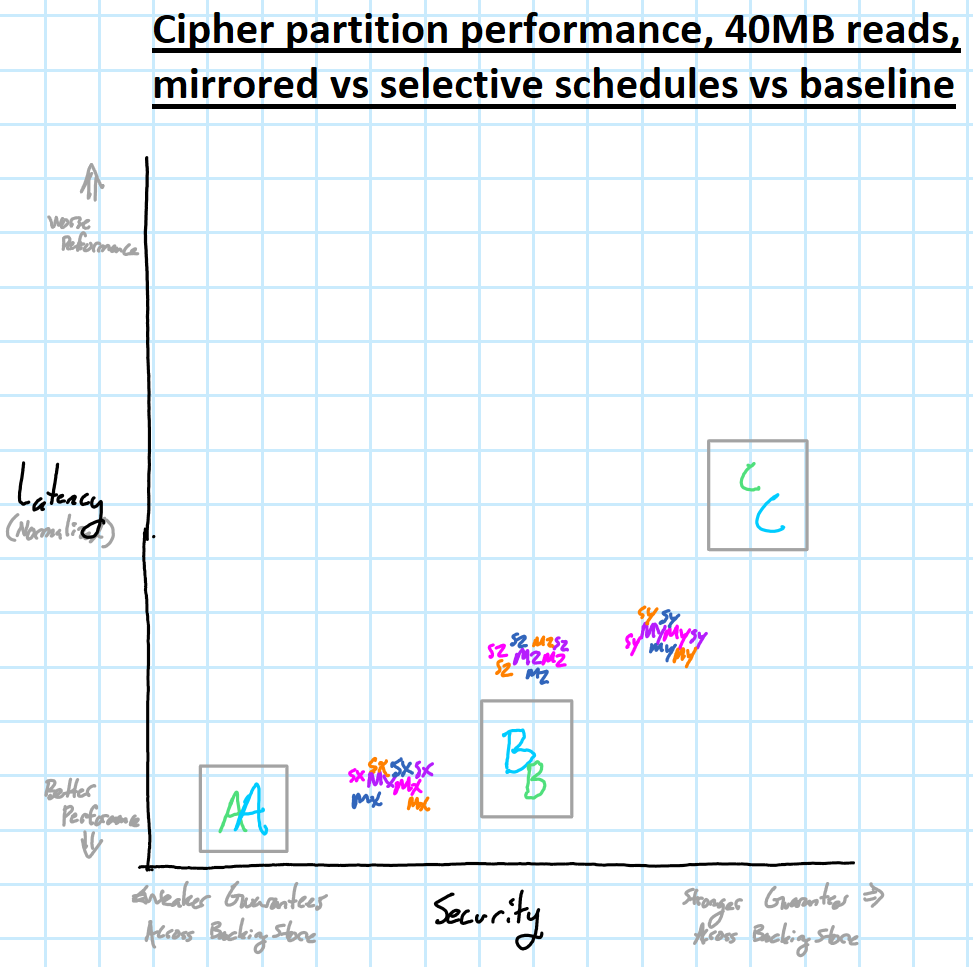
\includegraphics[width=\linewidth]{drawn/8.png}
   \caption{\TODO{Caption goes here}}\label{fig:mirrored-vs-selective}
\end{figure}

\subsection{Balancing Security Goals with a Constrained Energy Budget}

When our mobile devices enter power saving mode, it is usually because the total
energy/power budget for the device has become constrained for one reason or
another.

When a device enters this mode, all software and components are configured by
the OS to use as little of the available energy as possible. The filesystem
should be made to behave in a manner that is energy-aware as well.

Our goal is to use as little energy as possible (while reasonably preserving
filesystem performance) until the energy budget changes or the device dies.

Benefit: When constantly streaming data, e.g. using DLNA to stream a high
resolution video wirelessly to a TV on the same network, the ability to adapt to
time-varying data rates and QoS requirements while maintaining confidentiality
and integrity guarantees is paramount. This can be done by trading off a set of
security guarantees with respect to the energy spent crypting each bit. With
cipher switching, the filesystem can react dynamically to the system's total
energy budget while still aiming for the most performant (least latency)
configuration.
\TODO{See my earlier comment (in email or some other TODO) about reading vs. writing.  It seems fairly clear to me that you can make this work for writes, but I don't see hwo this works for reads. If the video is stored in a strong cipher, don't you have to decrypt it at that strength?  Where does the energy win come from on reads?}

\TODO{Need to include which strategy to use here and why (already typed up!)}

\begin{figure}[ht]
 \centering
  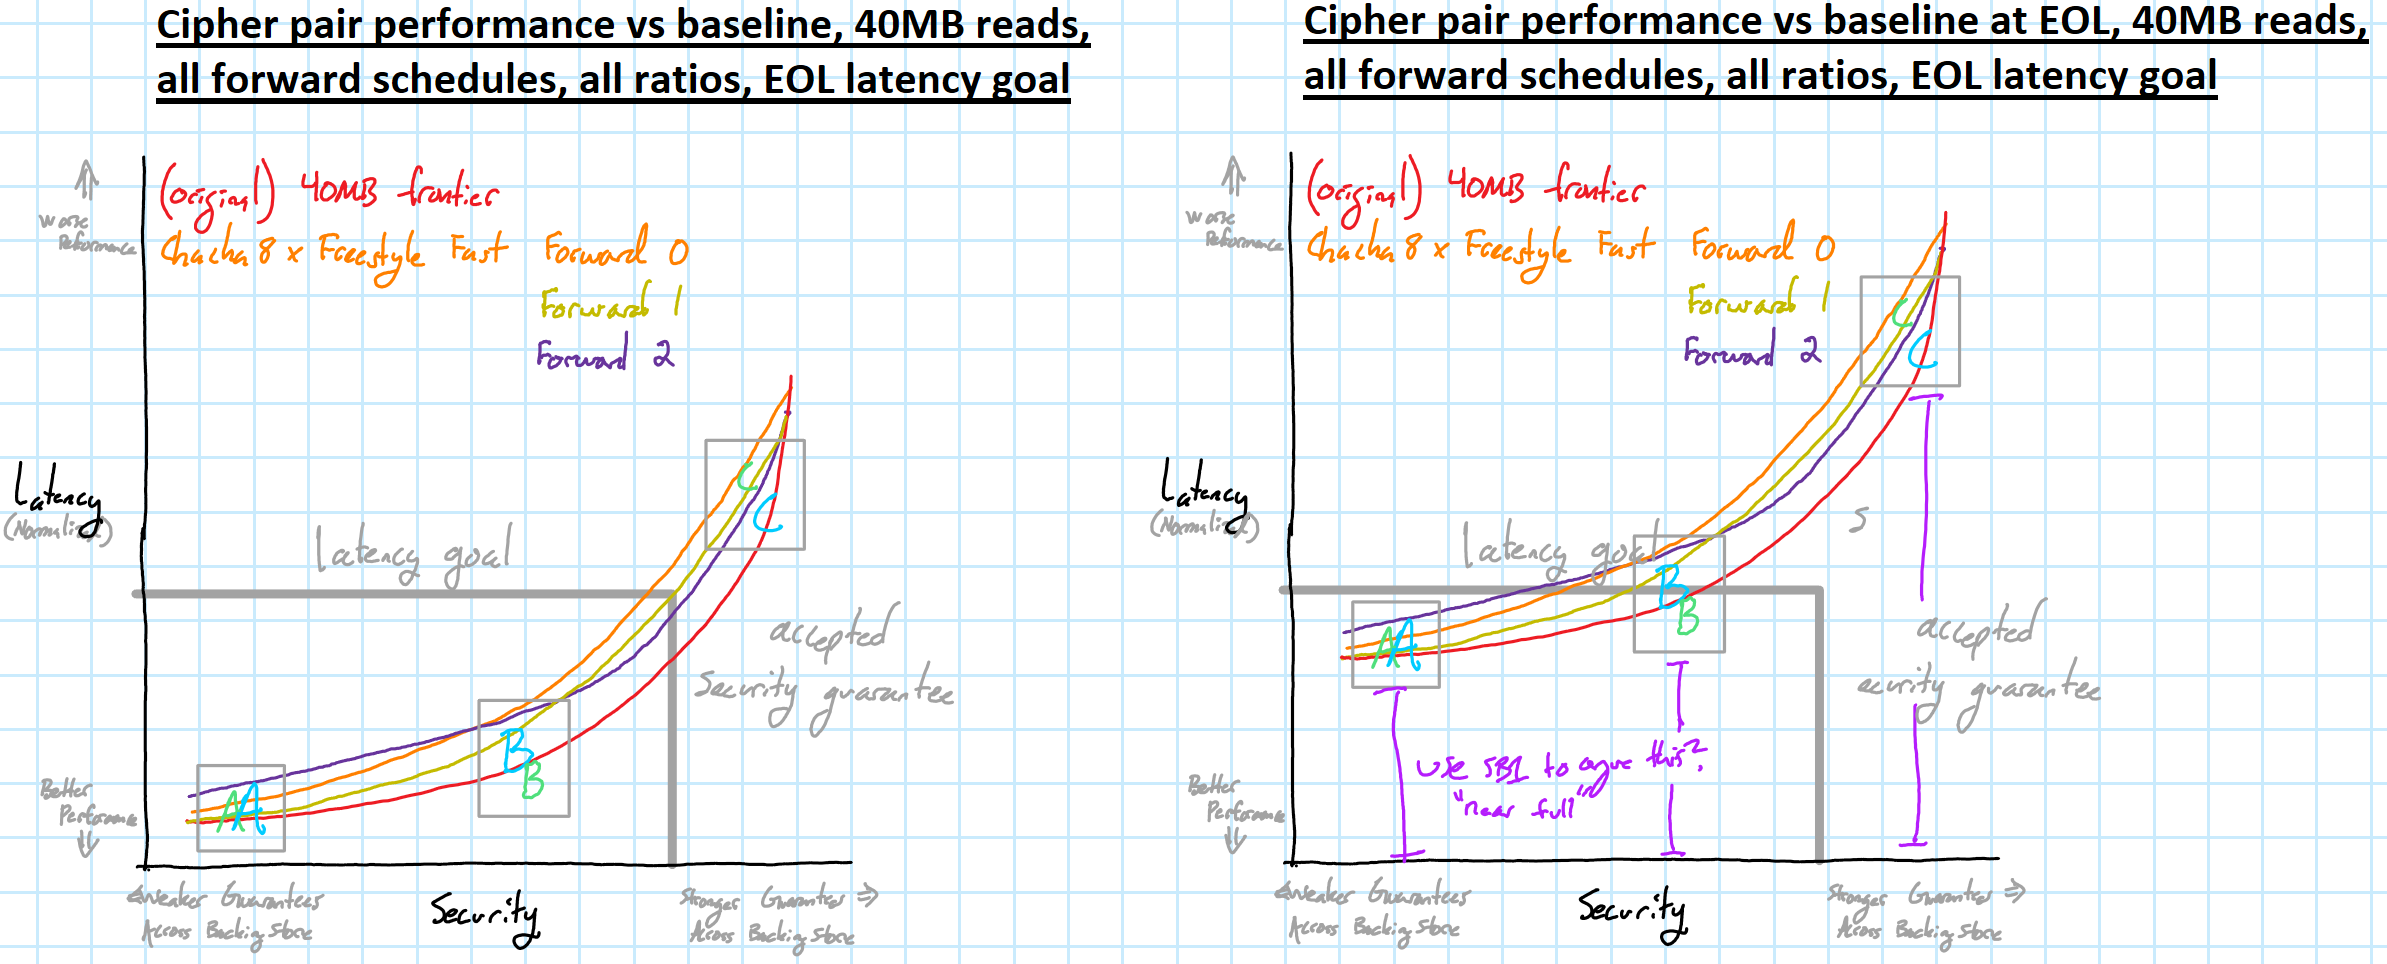
\includegraphics[width=\linewidth]{drawn/7.png}
   \caption{\TODO{Caption goes here}}\label{fig:energy-budget}
\end{figure}

\subsection{Responding to End-of-Life Slowdown in Solid State Drives}

Due to garbage collection and the append-mostly nature of SSDs and other NAND
devices, as free space becomes constrained, performance drops off a cliff. This
is a well-studied issue (see related work).

If the filesystem is made aware when the backing store is in such a state, we
can offset some of the (drastic) performance loss by switching the ciphers of hot
nuggets to the fastest cipher available until the disk space problem is
remedied, after which the system can detect return the swapped nuggets to their
former encrypted state.

Benefit: we can mitigate the performance loss of a slowing SSD by using a faster
but less secure cipher.

\begin{figure}[ht]
 \centering
  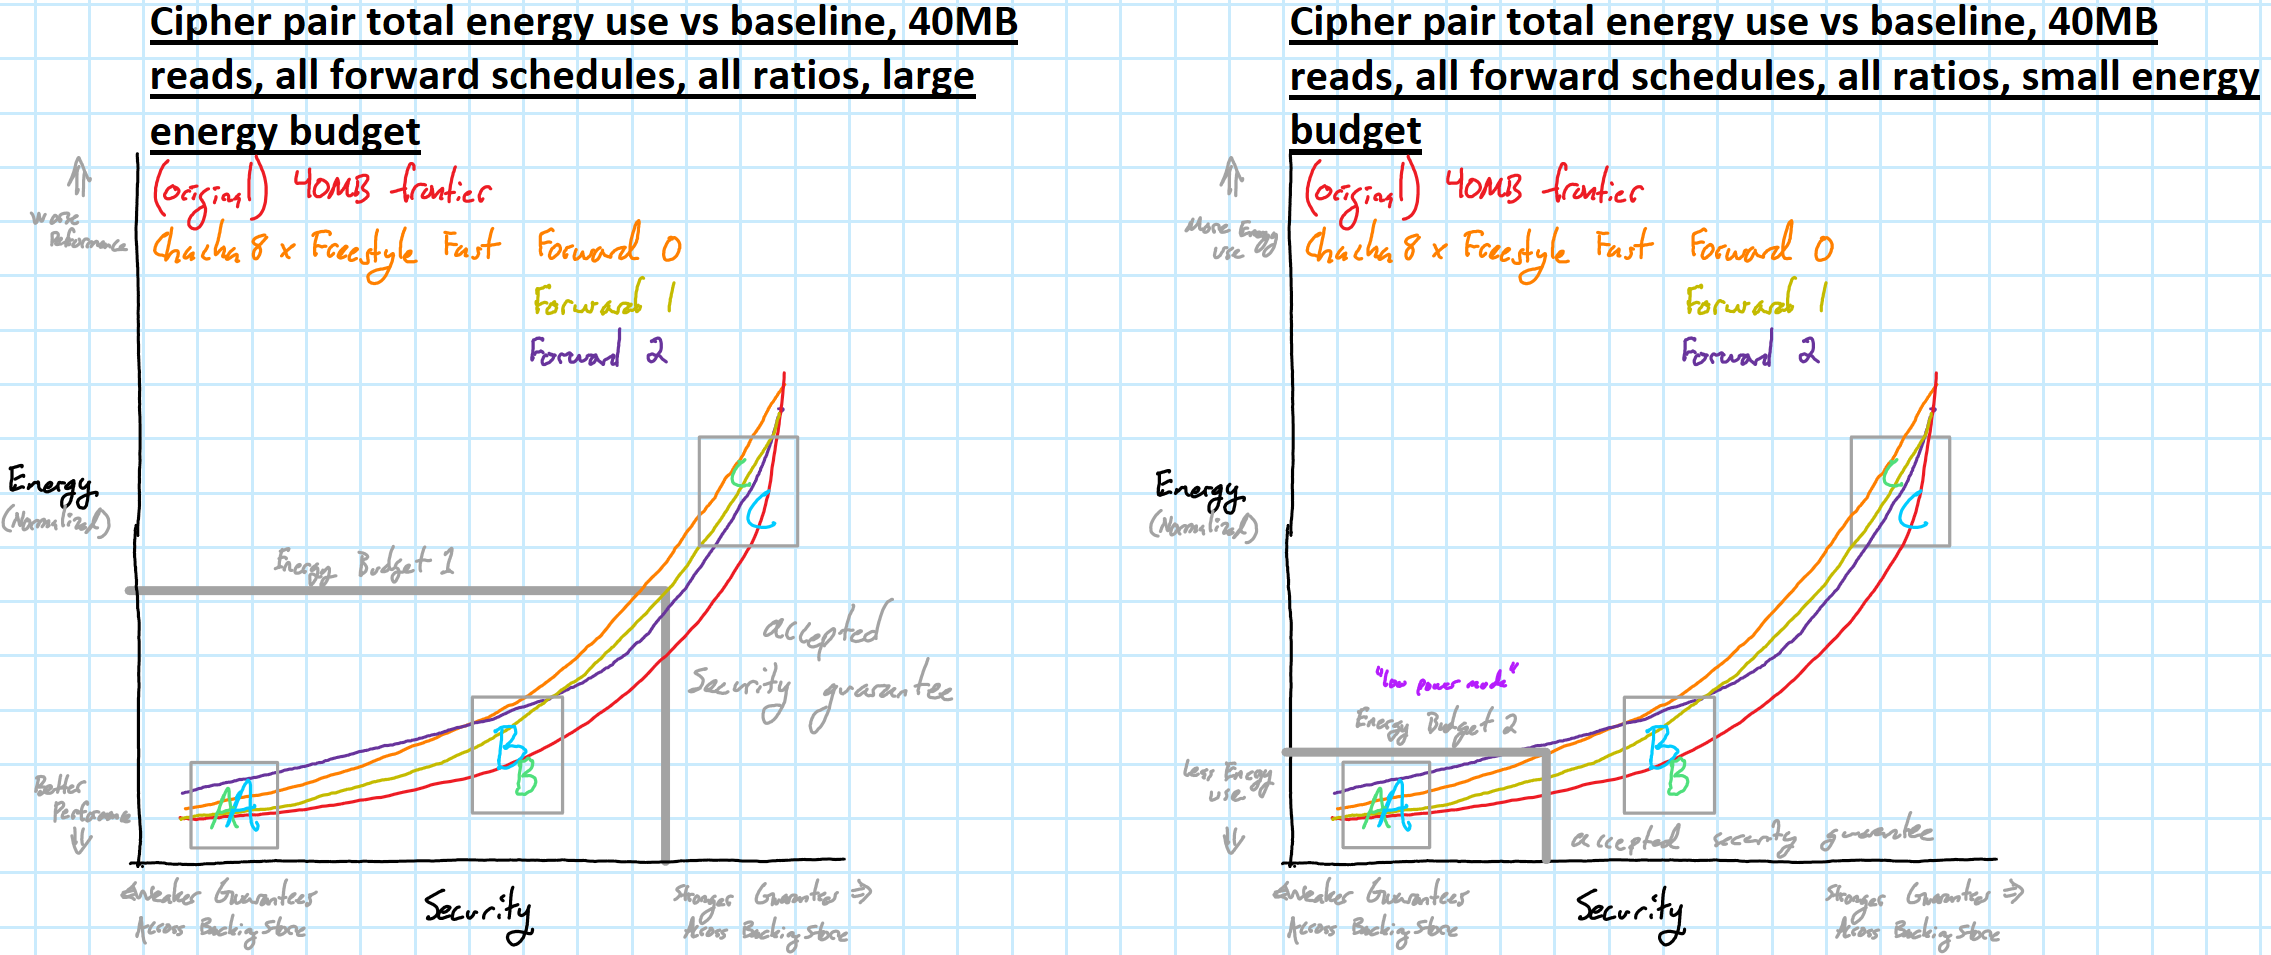
\includegraphics[width=\linewidth]{drawn/6.png}
   \caption{\TODO{Caption goes here}}\label{fig:eol}
\end{figure}

\subsection{Custody Panic: Securing Device Data Under Duress}

Nation-state and other adversaries have truly extensive compute resources at
their disposal, as well as knowledge of side-channels and access to technology
like q-bit computers.

Suppose one were attempting to re-enter a country through a border checkpoint
after visiting family when one is stopped. Your mobile device is confiscated and
placed in custody of the State. In such a scenario, it would be useful if the
device could swap itself into a more secure state as quickly as possible.

Benefit: greater security guarantee achieved using the highest security
encryption available versus powerful adversaries with unknown means and motive.

\TODO{Need to include which strategy to use here and why (already typed up!)}

\TODO{Dumb question: this scenario assumes you are worried about the data, but
can't wipe the drive, right?  Is that a plausible scenario? }
